\documentclass{beamer}

\usepackage{times}

\usepackage{hyperref}

\hypersetup{
  urlcolor=blue,
  linkcolor=blue,
  colorlinks=true
}

\usepackage{listings}
\lstset{frame=none, showstringspaces=false, basicstyle=\ttfamily\bfseries\footnotesize,
  xleftmargin=-8mm,language=Haskell,breaklines=true}

\title {Toward a Generative Framework for Safe Scientific Software}

\author{\textbf{Spencer Smith}}

\institute[McMaster University]
{
  Computing and Software Department\\
  Faculty of Engineering\\
  McMaster University
}

\date {
  Mar 17, 2026}

\subject{research software, software engineering, software
  quality, software safety, code and artifact generation, software documentation, assurance cases}
% This is only inserted into the PDF information catalog. Can be left
% out. 

\beamertemplatenavigationsymbolsempty 

\begin{document}

%%%%%%%%%%%%%%%%%%%%%%%%%%%%%%%%%%%%%%

\begin{frame}[plain]

\titlepage

% Thank Dr. Torngren (TURNgren) for invitation to join research meeting and the opportunity to speak
% Talk is about work in progress; I welcome feedback and discussion
% I will talk about Drasil, a generative framework for scientific software, and how we are working to add assurance case generation to Drasil
% scope is scientific computing software, but ideas would work for any well-understood software

\end{frame}

%%%%%%%%%%%%%%%%%%%%%%%%%%%%%%%%%%%%%% 

\begin{frame}

\frametitle{Favorite Thing About Stockholm -- Fika!}

% \begin{enumerate}
% \item Public transportation
% \item Safe feeling walking around the city
% \item Great dinners (\href{https://paganini.nu/} {Ristorante Paganini}, \href{https://www.krogguiden.se/restauranger/view/xiang-yue} {Xiang Yue}, \href{https://www.supper.nu/stockholm} {Supper})
% \item \href{https://tgt11.com/en/index.html?utm_source=google&utm_medium=cpc&utm_campaign=22020607672&gad_source=1&gad_campaignid=22016779082&gbraid=0AAAAADnuKU0qzms4rEx0ePOePCmMBK7kr&gclid=CjwKCAjwjtTNBhB0EiwAuswYhgdKEJiRTKsTD3MZyS_3rStQXaU3w5i6YGRWompmLwPLk6adt5hnYhoCgRYQAvD_BwE} {TGT11} (guitar store)
% \item Museums (Vasa, ABBA, Royal Palace, ...)
% \item Fika!
% \end{enumerate}

\includegraphics[width=1.0\textwidth]{./figures/Fika.pdf}

\end{frame}

%%%%%%%%%%%%%%%%%%%%%%%%%%%%%%%%%%%%%%

\begin{frame}

\frametitle{Toward a Generative Framework for Safe Scientific Software}

\begin{enumerate}
\item Drasil -- a gen framework for well-understood software
\item AC for computational medicine
\item Adding ACs to Drasil (work in progress)
\begin{itemize}
  \item Additional knowledge
  \item Additional infrastructure
\end{itemize}
\end{enumerate}

\end{frame}

%%%%%%%%%%%%%%%%%%%%%%%%%%%%%%%%%%%%%%

\begin{frame}

\frametitle{A Generative Framework for Scientific Software}

\begin{itemize}
\item \textbf{Goal} -- Improve qualities (e.g., safety, reliability, maintainability) of SS
\item \textbf{Idea}
  \begin{itemize}
  \item Adapt ideas from SE
  \item Document requirements, design, verification, AC, etc.
    \begin{itemize}
    \item Good -- improves quality
    \item Bad -- too much work, inevitable change, too hard to maintain
    \end{itemize}
  \end{itemize}
\item \textbf{Solution}
\begin{itemize}
\item Capture knowledge once
\item Generate all documentation and code
% \item Avoid duplication
% \item Traceability
% \item Reproducibility
\end{itemize}
\item \textbf{Implement Solution --
    \href{https://github.com/JacquesCarette/Drasil} {Drasil}}
  \begin{itemize}
  \item Facilitates change
  \item Traceability
  \item Reproducibility
  \item Sustainability
  \item Certification
  \item Captures best practices
  \end{itemize}
\end{itemize}

\end{frame}

%%%%%%%%%%%%%%%%%%%%%%%%%%%%%%%%%%%%%%

\begin{frame}

\frametitle{GlassBR}

\begin{columns}
\begin{column}{0.5\textwidth}

\includegraphics[width=1.0\textwidth]{./figures/physicalsystimage.png}
\end{column}
\begin{column}{0.5\textwidth}
Given

\begin{itemize}
\item dimensions of glass plane
\item glass type
\item explosion characteristics
\item tolerable breakage probability
\end{itemize}

Predict whether the glass will withstand the explosion

\end{column}
\end{columns}

\end{frame}

%%%%%%%%%%%%%%%%%%%%%%%%%%%%%%%%%%%%%%

\begin{frame}

%\frametitle{Input Knowledge}

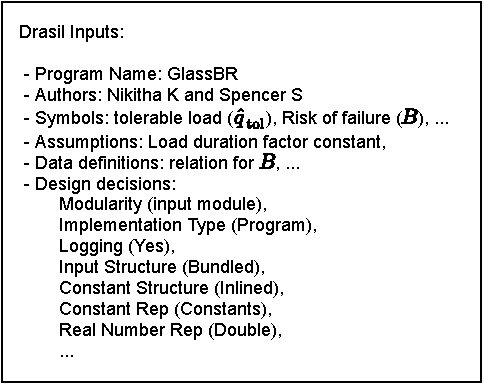
\includegraphics[width=0.95\textwidth]{./figures/DrasilInputs.pdf}

\end{frame}

%%%%%%%%%%%%%%%%%%%%%%%%%%%%%%%%%%%%%%

\begin{frame}

%\frametitle{Input Knowledge}

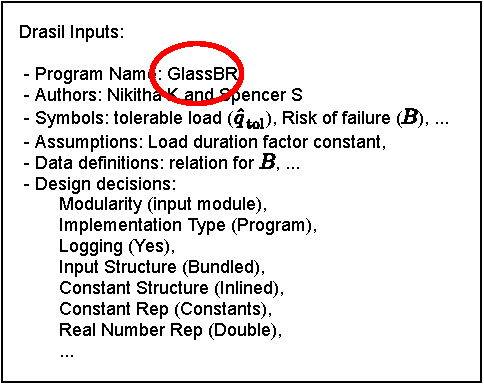
\includegraphics[width=0.95\textwidth]{./figures/InputsCircleGlassBR.pdf}

\end{frame}

%%%%%%%%%%%%%%%%%%%%%%%%%%%%%%%%%%%%%%

\begin{frame}

%\frametitle{Input Knowledge}

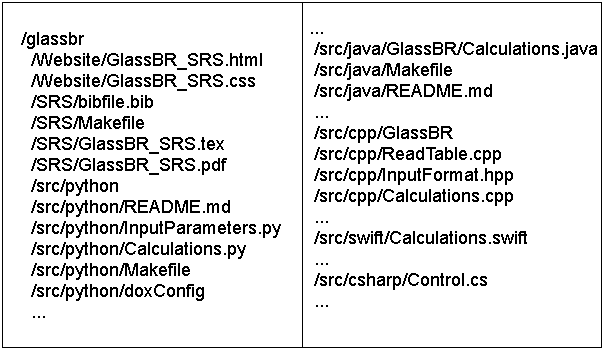
\includegraphics[width=1.05\textwidth]{./figures/FoldersFiles.pdf}

\end{frame}

%%%%%%%%%%%%%%%%%%%%%%%%%%%%%%%%%%%%%%

\begin{frame}

%\frametitle{Input Knowledge}

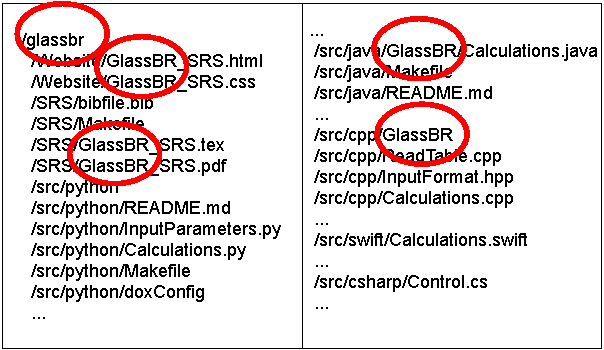
\includegraphics[width=1.05\textwidth]{./figures/FoldersFilesCircleGlassBR.pdf}

\end{frame}

%%%%%%%%%%%%%%%%%%%%%%%%%%%%%%%%%%%%%%

\begin{frame}

%\frametitle{Input Knowledge}

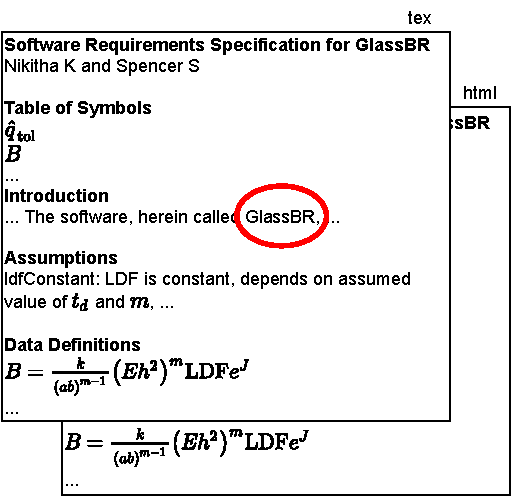
\includegraphics[width=1.05\textwidth]{./figures/SRSCircleGlassBR.pdf}

\end{frame}

%%%%%%%%%%%%%%%%%%%%%%%%%%%%%%%%%%%%%%

\begin{frame}

%\frametitle{Input Knowledge}

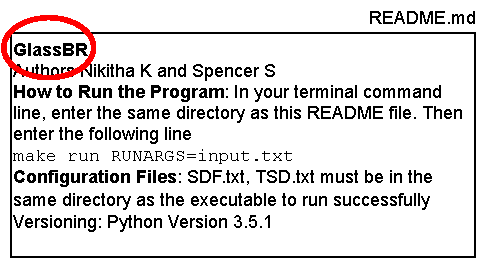
\includegraphics[width=1.05\textwidth]{./figures/READMECircleGlassBR.pdf}

\end{frame}

%%%%%%%%%%%%%%%%%%%%%%%%%%%%%%%%%%%%%%

\begin{frame}

%\frametitle{Input Knowledge}

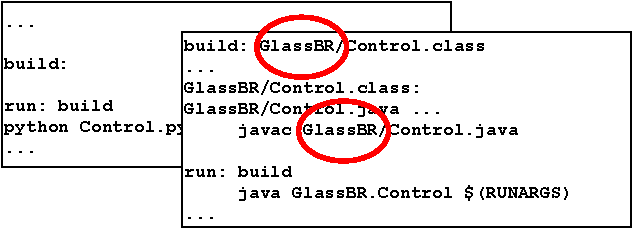
\includegraphics[width=1.05\textwidth]{./figures/MakefileCircleGlassBR.pdf}

\end{frame}

%%%%%%%%%%%%%%%%%%%%%%%%%%%%%%%%%%%%%%

\begin{frame}

%\frametitle{Input Knowledge}

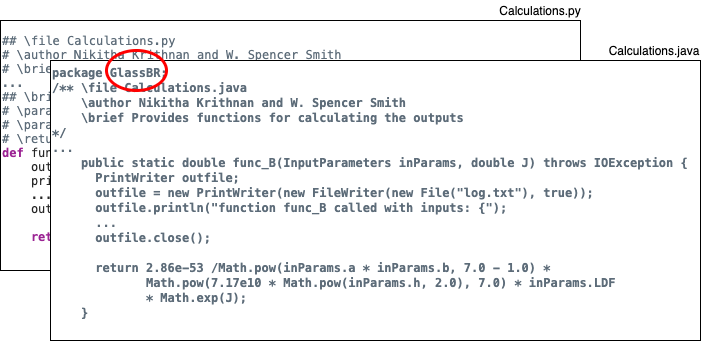
\includegraphics[width=1.05\textwidth]{./figures/CodeCircleGlassBR.png}

\end{frame}

%%%%%%%%%%%%%%%%%%%%%%%%%%%%%%%%%%%%%%

\begin{frame}

\frametitle{$J_{\mbox{tol}}$ in SRS.pdf}
\begin{center}

\includegraphics[width=0.9\textwidth]{./figures/Jtol_pdf.pdf}
\end{center}
\end{frame}

%%%%%%%%%%%%%%%%%%%%%%%%%%%%%%%%%%%%%

\begin{frame}[plain, fragile]

\frametitle{$J_{\mbox{tol}}$ in SRS.tex}
~\\
\begin{lstlisting}
...
Label & Stress distribution factor (Function) based on Pbtol
        
\\ \midrule \\
Symbol & ${J_{\text{tol}}}$
         
\\ \midrule \\
Units & Unitless
        
\\ \midrule \\
Equation & \begin{displaymath}
           {J_{\text{tol}}}=\ln\left(\ln\left(\frac{1}{1-{P_{\text{b}\text{tol}}}}\right) \frac{\left(\frac{a}{1000} \frac{b}{1000}\right)^{m-1}}{k \left(E\cdot{}1000 \left(\frac{h}{1000}\right)^{2}\right)^{m} LDF}\right)
           \end{displaymath}
\\ \midrule \\
Description & ...
\end{lstlisting}
\end{frame}

%%%%%%%%%%%%%%%%%%%%%%%%%%%%%%%%%%%%%%

\begin{frame}[plain, fragile]

\frametitle{$J_{\mbox{tol}}$ in SRS.html}

\begin{lstlisting}

...
<th>Equation</th>
<td>
\[{J_{\text{tol}}}=\ln\left(\ln\left(\frac{1}{1-{P_{\text{b}\text{tol}}}}\right) \frac{\left(\frac{a}{1000} \frac{b}{1000}\right)^{m-1}}{k \left(E\cdot{}1000 \left(\frac{h}{1000}\right)^{2}\right)^{m} LDF}\right)\]
</td>
...
\end{lstlisting}

\end{frame}
%%%%%%%%%%%%%%%%%%%%%%%%%%%%%%%%%%%%%

\begin{frame}[plain, fragile]

\frametitle{$J_{\mbox{tol}}$ in Python}

\begin{lstlisting}
## \brief Calculates stress distribution factor (Function) based on Pbtol
# \param inParams structure holding the input values
# \return stress distribution factor (Function) based on Pbtol
def func_J_tol(inParams):
    outfile = open("log.txt", "a")
    print("function func_J_tol called with inputs: {", file=outfile)
    print("  inParams = ", end="", file=outfile)
    print("Instance of InputParameters object", file=outfile)
    print("  }", file=outfile)
    outfile.close()
    
    return math.log(math.log(1.0 / (1.0 - inParams.P_btol)) * ((inParams.a / 1000.0 * (inParams.b / 1000.0)) ** (7.0 - 1.0) / (2.86e-53 * (7.17e10 * 1000.0 * (inParams.h / 1000.0) ** 2.0) ** 7.0 * inParams.LDF)))
\end{lstlisting}
\end{frame}

%%%%%%%%%%%%%%%%%%%%%%%%%%%%%%%%%%%%%%

\begin{frame}[plain, fragile]

\frametitle{$J_{\mbox{tol}}$ in Java}

\begin{lstlisting}
    /** \brief Calculates stress distribution factor (Function) based on Pbtol
        \param inParams structure holding the input values
        \return stress distribution factor (Function) based on Pbtol
    */
    public static double func_J_tol(InputParameters inParams) throws IOException {
        PrintWriter outfile;
        outfile = new PrintWriter(new FileWriter(new File("log.txt"), true));
        ...
        return Math.log(Math.log(1.0 / (1.0 - inParams.P_btol)) * (Math.pow(inParams.a / 1000.0 * (inParams.b / 1000.0), 7.0 - 1.0) / (2.86e-53 * Math.pow(7.17e10 * 1000.0 * Math.pow(inParams.h / 1000.0, 2.0), 7.0) * inParams.LDF)));
    }
\end{lstlisting}
\end{frame}

%%%%%%%%%%%%%%%%%%%%%%%%%%%%%%%%%%%%%%

\begin{frame}[plain, fragile]

\frametitle{$J_{\mbox{tol}}$ in Drasil (Haskell)}

\begin{lstlisting}

tolStrDisFacEq :: Expr
tolStrDisFacEq = ln (ln (recip_ (exactDbl 1 $- sy pbTol))
  `mulRe` (((sy plateLen $/ exactDbl 1000) `mulRe` (sy plateWidth $/ exactDbl 1000)) $^ (sy sflawParamM $- exactDbl 1) $/
    (sy sflawParamK `mulRe` ((sy modElas `mulRe` exactDbl 1000 `mulRe`
    square (sy minThick $/ exactDbl 1000)) $^ sy sflawParamM) `mulRe` sy lDurFac)))

\end{lstlisting}
\end{frame}

%%%%%%%%%%%%%%%%%%%%%%%%%%%%%%%%%%%%%%

\begin{frame}[plain, fragile]

\frametitle{$J_{\mbox{tol}}$ without Unit Conversion}

\begin{lstlisting}
tolStrDisFacEq :: Expr
tolStrDisFacEq = ln (ln (recip_ (exactDbl 1 $- sy pbTol))
  `mulRe` ((sy plateLen `mulRe` sy plateWidth) $^ (sy sflawParamM $- exactDbl 1) $/
    (sy sflawParamK `mulRe` ((sy modElas `mulRe`
    square (sy minThick)) $^ sy sflawParamM) `mulRe` sy lDurFac)))
\end{lstlisting}
\end{frame}

%%%%%%%%%%%%%%%%%%%%%%%%%%%%%%%%%%%%%%

% \begin{frame}

% %\frametitle{Input Knowledge}

% 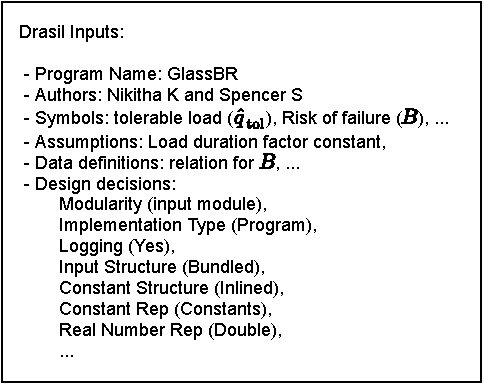
\includegraphics[width=0.95\textwidth]{./figures/DrasilInputs.pdf}

% \end{frame}

%%%%%%%%%%%%%%%%%%%%%%%%%%%%%%%%%%%%%%

\begin{frame}


\includegraphics[width=1.0\textwidth]{./figures/DrasilSupportsChange.png}

\end{frame}

%%%%%%%%%%%%%%%%%%%%%%%%%%%%%%%%%%%%%%

\begin{frame}

\frametitle{What Drasil Can Currently Do}

\begin{itemize}
  \item Explicit relations, LHS = ...
  \item Systems of higher-order ODEs
  \item Knowledge on rigid body mechanics, heat transfer
  \item SRS (LaTeX, html, MD books)
  \item Code (Python, C++, C sharp, Java, Swift), Jupyter notebooks
  \item README files, Makefile
  \item Doxygen comments
  \item Infrastructure for knowledge about people
\end{itemize}

\end{frame}

%%%%%%%%%%%%%%%%%%%%%%%%%%%%%%%%%%%%%%

\begin{frame}

\frametitle{Advantages of AC Generation}

\begin{itemize}
  \item Build AC and software together
  \item Facilitates change
  \item Traceability
  \item Reuse of common knowledge
  \item Design space exploration
\end{itemize}

\end{frame}

%%%%%%%%%%%%%%%%%%%%%%%%%%%%%%%%%%%%%%

%\hoffset=-.4in
\begin{frame}[plain, fragile]

\frametitle{AC Example for Computational Medicine}

\begin{center}
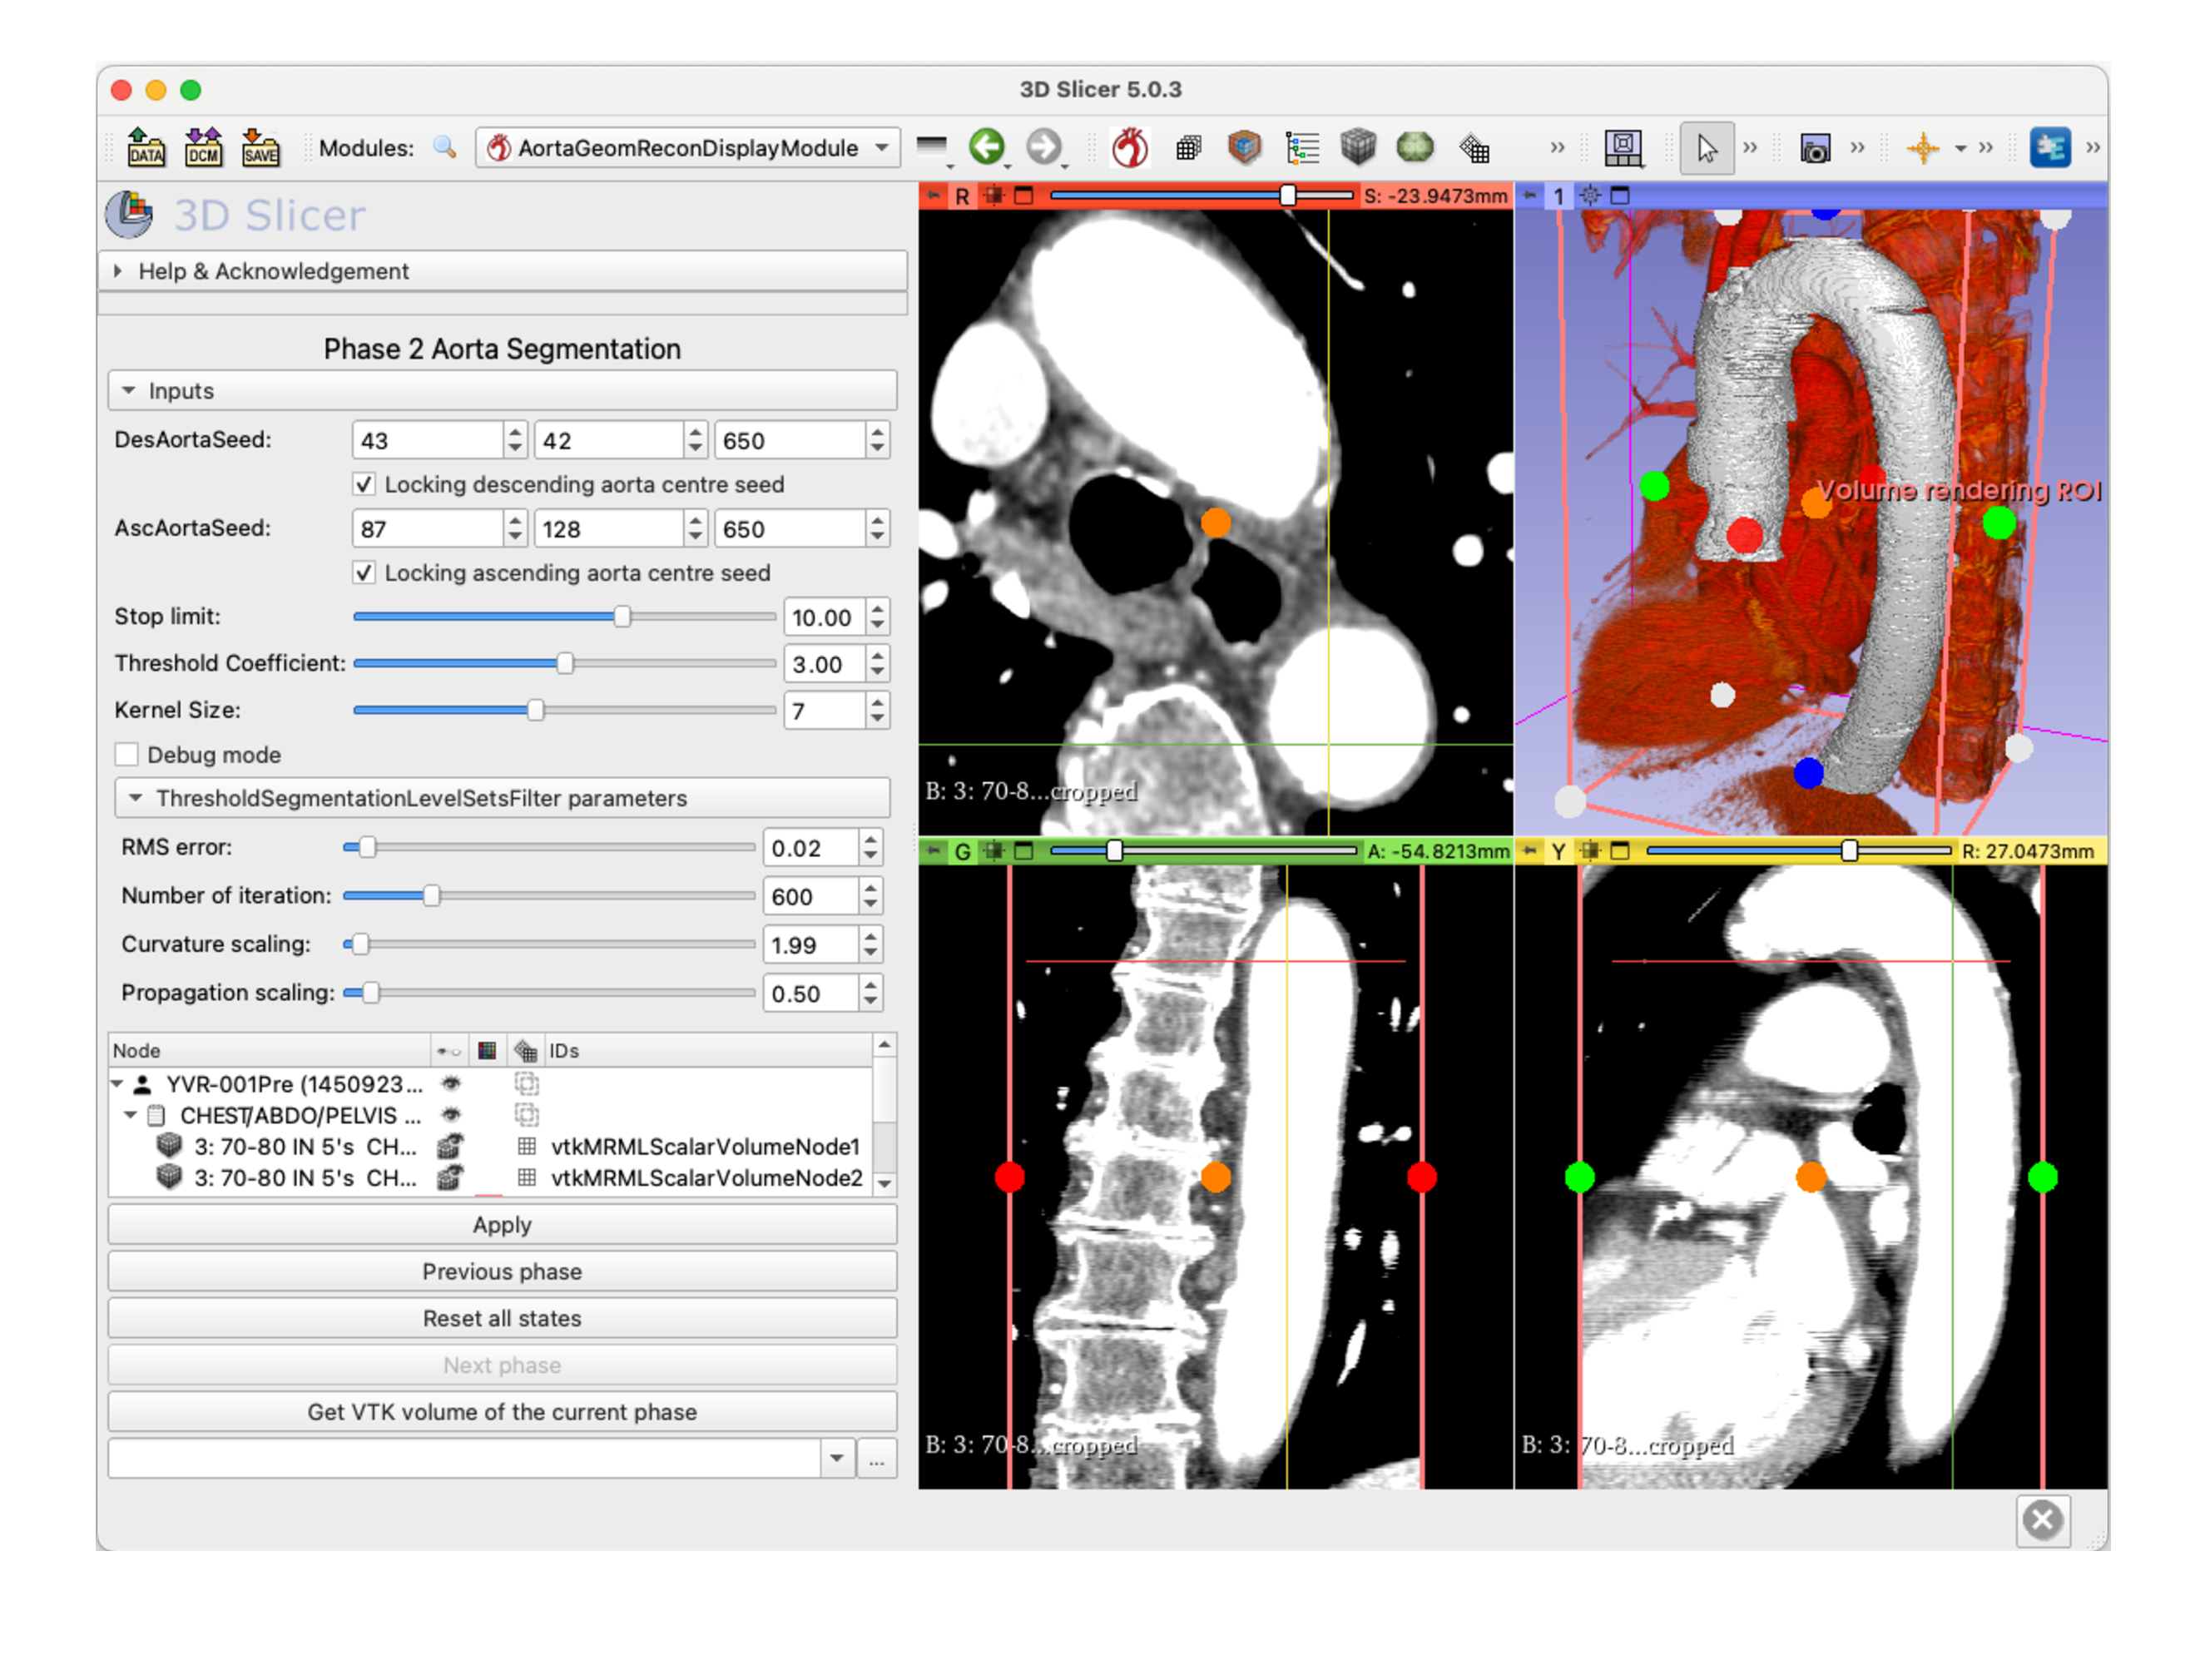
\includegraphics[scale=0.27]{./figures/AGR_Screenshot.pdf}
\end{center}
% how determine how to invest time - what is required
\end{frame}
%\hoffset=0in
%%%%%%%%%%%%%%%%%%%%%%%%%%%%%%%%%%%%%%

%\hoffset=-.3in
\begin{frame}[plain, fragile]

%\frametitle{Top Level Argument}

\begin{center}
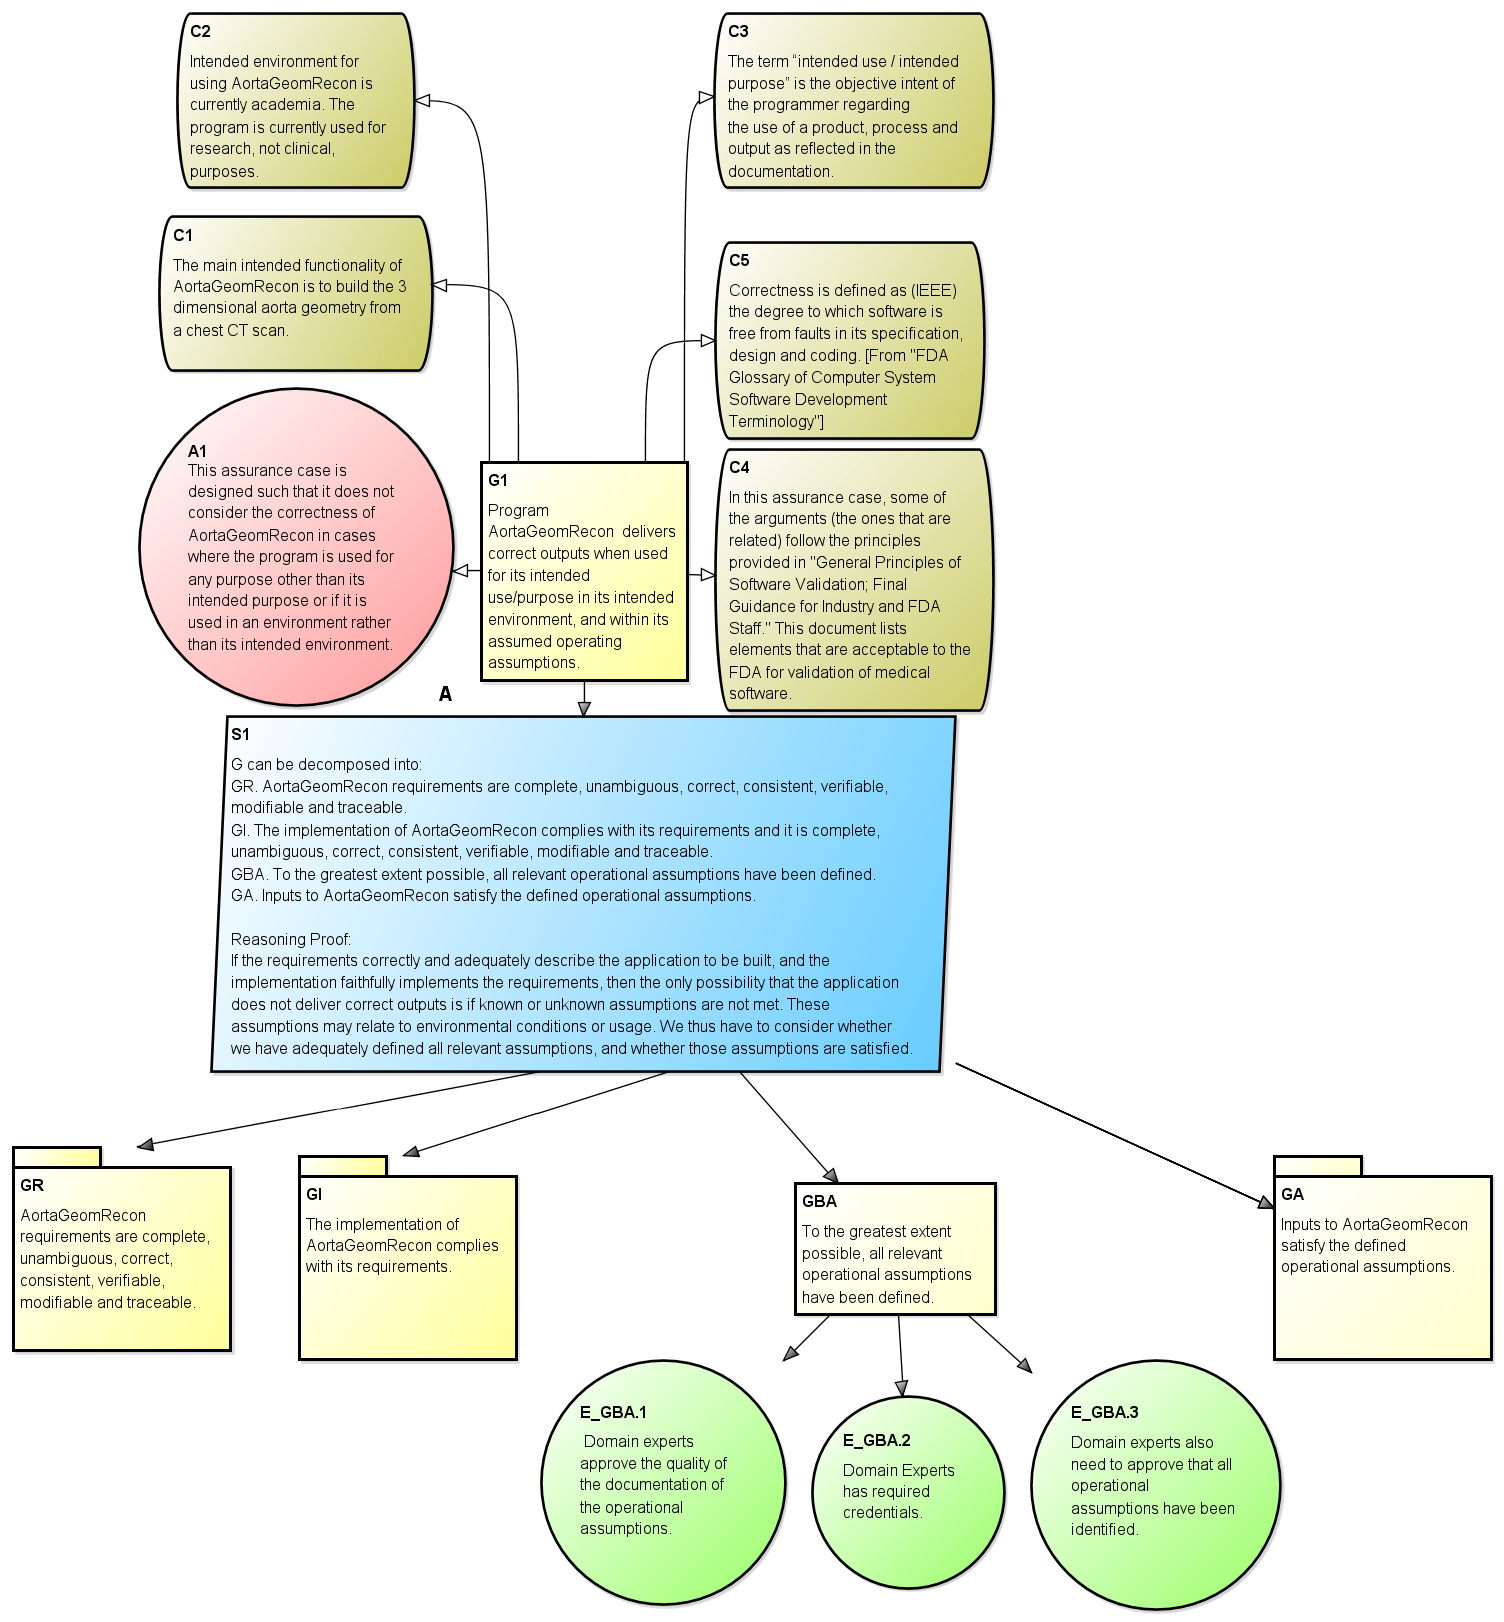
\includegraphics[scale=0.2]{./figures/Top_Level.png}
\end{center}
% argument for SRS - need to know that model is valid
% argument for code - need to know that code matches the model
% central role of assumptions, scope decisions, modelling decisions
% generation of testing code
\end{frame}
%\hoffset=0in

%%%%%%%%%%%%%%%%%%%%%%%%%%%%%%%%%%%%%%

% %\hoffset=-.68in
% \begin{frame}[plain, fragile]

% %\frametitle{Evidence}

% %\begin{center}
% %\hspace{-0.7in}
% 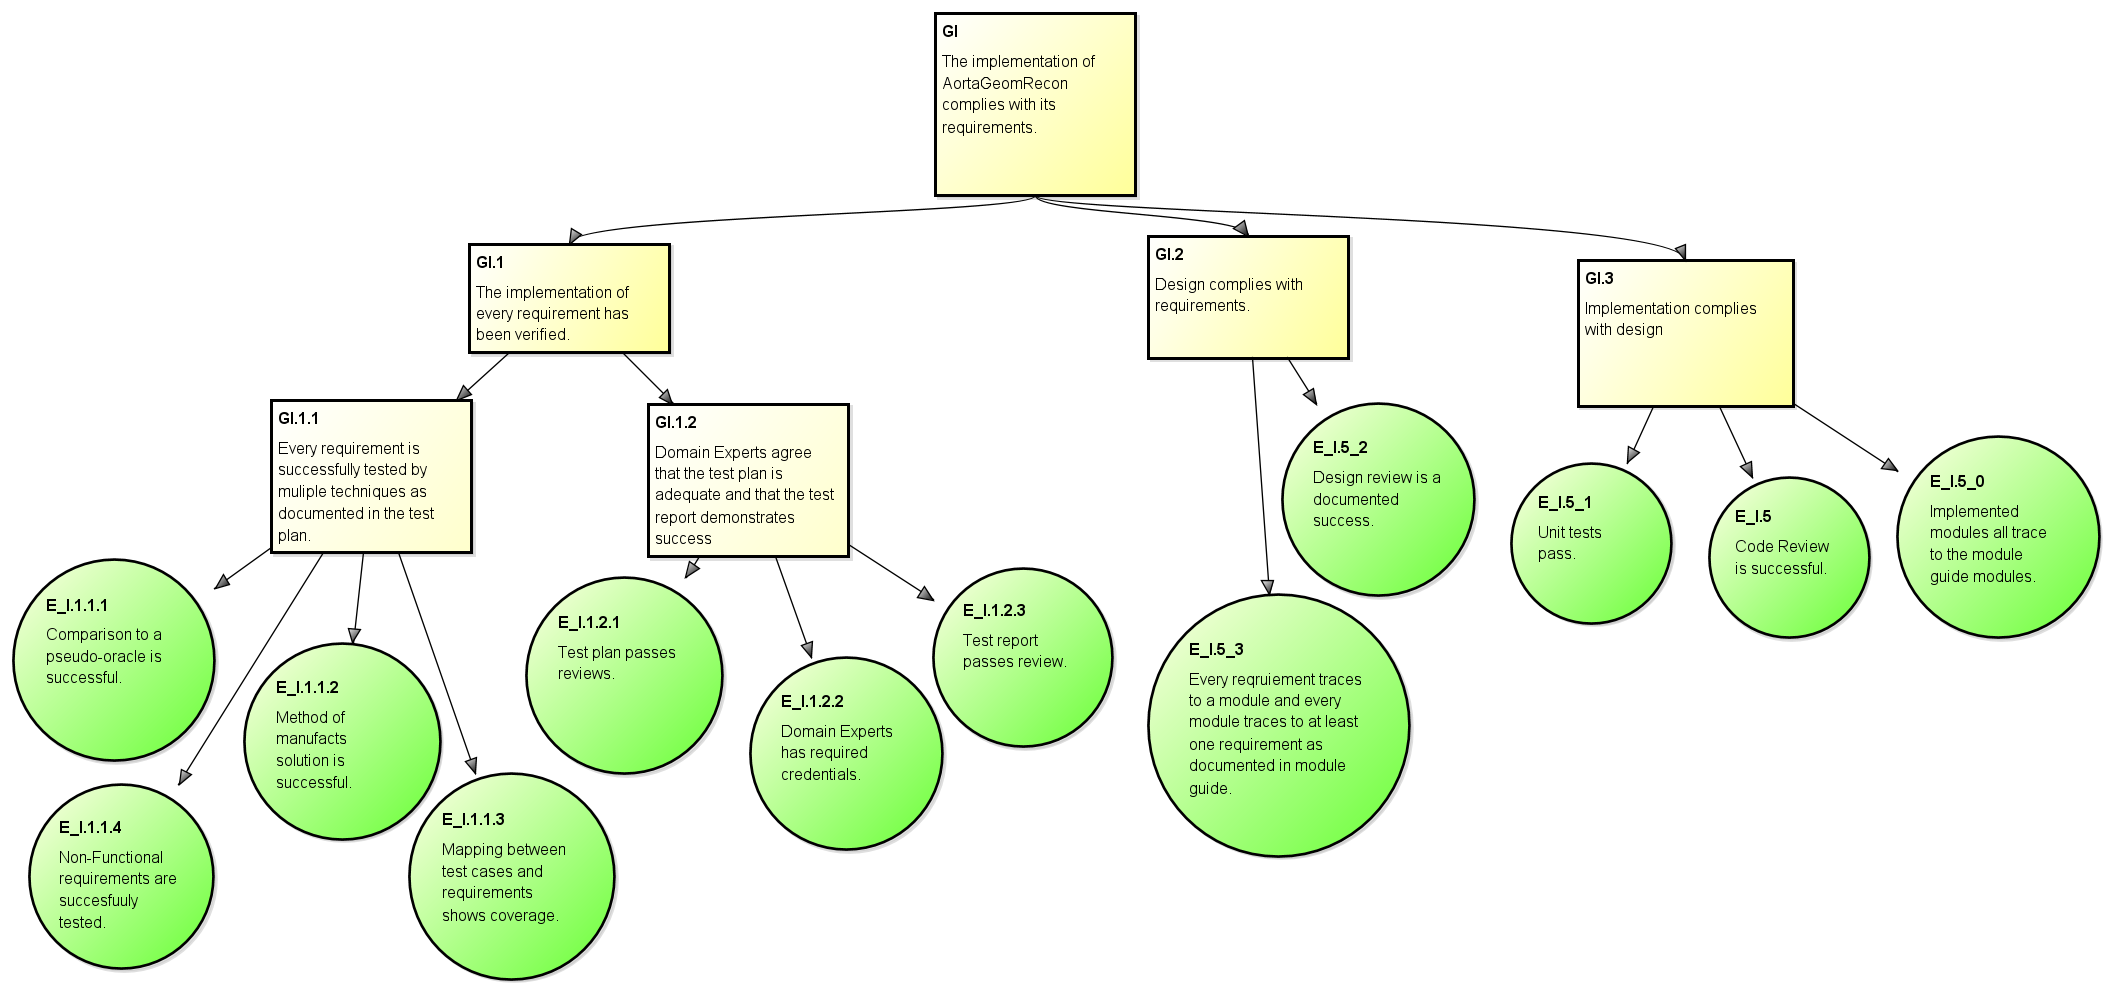
\includegraphics[scale=0.21]{./figures/GSN_GI.png}
% %\end{center}

% %\citep{SmithAndLin2024_arXiv}
% \end{frame}
% %\hoffset=0in

%%%%%%%%%%%%%%%%%%%%%%%%%%%%%%%%%%%%%%

\begin{frame}

\frametitle{Required Additions to Drasil for ACs}

\begin{itemize}
  \item Additional Knowledge
  \begin{itemize}
    \item Generation of GSN diagrams
    \item Reviewer reports
    \item Test case generation
  \end{itemize}
  \item Additional infrastructure
  \begin{itemize}
    \item Rationale/evidence for decisions and assumptions
    \item Theories and theory refinement
  \end{itemize}
\end{itemize}

\end{frame}

%%%%%%%%%%%%%%%%%%%%%%%%%%%%%%%%%%%%%%

\begin{frame}

\frametitle{Projectile Motion Example}

\hspace{-0.5in}
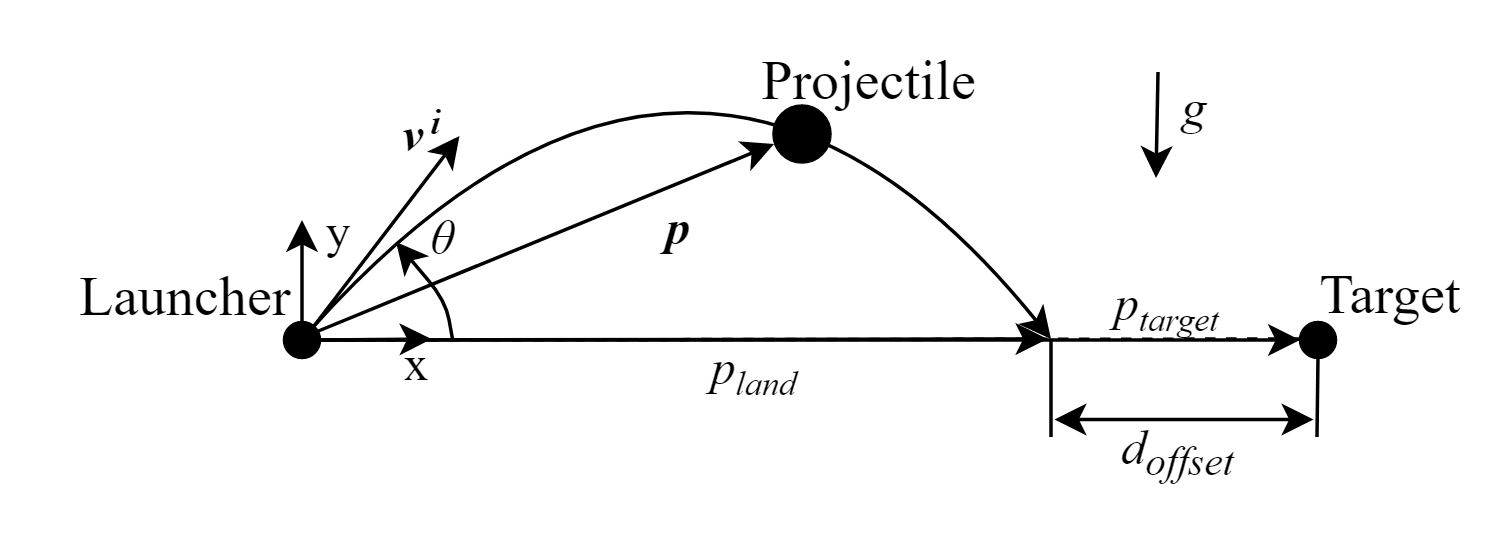
\includegraphics[scale=0.6]{./figures/Launch.jpg}
~\\
\href{https://github.com/smiths/caseStudies/blob/master/CaseStudies/projectile/projectileSRS_RefinedTheories/Projectile_SRS.pdf} {(WIP) SRS.pdf}

\end{frame}
%%%%%%%%%%%%%%%%%%%%%%%%%%%%%%%%%%%%%%

\begin{frame}[allowframebreaks]

\frametitle{Validity of Model}
%comment on rationale
\begin{itemize}
\item Scope Decisions
\begin{itemize}
  \item Orientation of projectile ignored
  \item Only kinematic equations (no forces)
\end{itemize}
\item Modelling Decisions
\begin{itemize}
  \item Cartesian coordinate system
  \item $y$ axis opposite to gravity
  \item Launcher at origin
  \item Target on $x$ axis
  \item Positive $x$ direction from launcher to target
  \item Time starts at zero
  \item Launch velocity is positive
  \item Magnitude and angle rep.\ for initial velocity
\end{itemize}
\item Data constraints
\begin{itemize}
  \item Inputs
  \begin{itemize}
  \item $p_\text{target} > 0$
  \item $v_\text{launch} > 0$
  \item $0 < \theta < \frac{\pi}{2}$ 
  \item 
  \end{itemize}
  \item Outputs
  \begin{itemize}
  \item $p_\text{land} > 0$
  \item $d_\text{offset} > -p_\text{target}$
  \item $t_\text{flight} > 0$
  \end{itemize}
\end{itemize}

\item Helper Assumptions
\begin{itemize}
  \item The motion of the particle is one dimensional
  \item The acceleration is constant
\end{itemize}
\item Generic Assumptions
\begin{itemize}
  \item The variables only depend on two dimensions
  \item The acceleration is constant in the $x$ direction
  \item The acceleration is constant in the $y$ direction
  \item The acceleration is due to gravity
\end{itemize}
\item Projectile Specific Assumptions
\begin{itemize}
  \item The acceleration in the $x$-direction is zero
  \item The constant acceleration in the $y$-direction is due to gravity
  \item The constant acceleration in the $y$-direction is $-9.8$ m/s$^2$
  \item There are no obstructions to impede the projectile's motion
  \item The surface of the planet is flat (no curvature)
\end{itemize}
\item Rationale Assumptions
\begin{itemize}
  \item Only care about the motion of the centre of mass of the projectile
  \item Distance is small enough that curvature can be neglected
  \item Air drag is neglected
  \item The rotation of the planet is neglected
\end{itemize}
\end{itemize}

\end{frame}
%%%%%%%%%%%%%%%%%%%%%%%%%%%%%%%%%%%%%%

\begin{frame}

\frametitle{Concluding Remarks}

\begin{itemize}
\item Generate assurance cases for models, numerical algorithms and code implementation
\item Add ACs to Drasil
\item Modelling decisions/assumptions
\begin{itemize}
  \item Scope decisions
  \item Modelling decisions
  \item Data constraints
  \item Assumptions
\end{itemize}
\item Justify model via an AC
\begin{itemize}
  \item Rationale
  \item Evidence (possibly via generation of test cases)
\end{itemize}
\item Justify numerical algorithm via an AC
\item Little theories, theory refinement
\item Propagation of modelling decisions/assumptions through theories
\item Measure and regenerate
\end{itemize}

\end{frame}

%%%%%%%%%%%%%%%%%%%%%%%%%%%%%%%%%%%%%%

\end{document}